
\documentclass[aspectratio=1610]{beamer}

\usepackage[utf8]{inputenc}
\usepackage[T1]{fontenc}
\usepackage{amsmath,amssymb,amsfonts}
\usepackage{hyperref} % before url package otherwise there is a pb
\usepackage{url}

\setbeamertemplate{navigation symbols}{%
    \usebeamerfont{footline}%
    \usebeamercolor[fg]{footline}%
    \hspace{1em}%
    \insertframenumber/\inserttotalframenumber
}
\setbeamercolor{footline}{fg=black}


\usepackage{comment}

\usepackage{algorithmic}
\usepackage[ruled,noline,noend]{algorithm2e}
\algomargin 0pt
\SetAlCapHSkip{0pt}
\DontPrintSemicolon
\SetKw{Continue}{continue}
% fix bug in algorithm2e
\makeatletter
\renewcommand{\@algocf@start}{%
  \@algoskip%
  \begin{lrbox}{\algocf@algobox}%
  \setlength{\algowidth}{\hsize}%
  \vbox\bgroup% save all the algo in a box
  \hbox to\algowidth\bgroup\hbox to \algomargin{\hfill}\vtop\bgroup%
  \ifthenelse{\boolean{algocf@slide}}{\parskip 0.5ex\color{black}}{}%
  % initialization
  \addtolength{\hsize}{-\algomargin}%
  % we don't want our algorithm lines numbered, so let's ditch that right
  % space.
  % \addtolength{\hsize}{-1.5em}% 1.5em to let space for line numbering
  \let\@mathsemicolon=\;\def\;{\ifmmode\@mathsemicolon\else\@endalgoln\fi}%
  \raggedright%
  \AlFnt{}%
  \ifthenelse{\boolean{algocf@slide}}{\IncMargin{\skipalgocfslide}}{}%
  \@algoinsideskip%
%   \let\@emathdisplay=\]\def\]{\algocf@endline\@emathdisplay\nl}%
}%
\makeatother

\usepackage{tikz}
\usetikzlibrary{calc, positioning, arrows.meta}
\usetikzlibrary{shapes.geometric} % for ellipse
\usetikzlibrary{arrows}
\usetikzlibrary{positioning}
\tikzset{
  state/.style={
    rectangle,
    rounded corners,
    draw=black, thick,
    minimum height=2em,
    inner sep=2pt,
    text centered,
  },
}
\usetikzlibrary{tikzmark}
\usepackage{pgfplots}

\usepackage{multirow}
\usepackage{multicol}

\newcommand{\NN}{\ensuremath{\mathbb N}}
\newcommand{\ZZ}{\ensuremath{\mathbb Z}}
\newcommand{\QQ}{\ensuremath{\mathbb{Q}}}
\newcommand{\RR}{\ensuremath{\mathbb{R}}}
\newcommand{\CC}{\ensuremath{\mathbb{C}}}
\newcommand{\K}{\ensuremath{\mathbb{K}}}
\newcommand{\PP}{\ensuremath{\mathbb{P}}} % for projective line
\newcommand{\FF}{\ensuremath{\mathbb F}}
\newcommand{\F}{\ensuremath{\mathbb F}}
\newcommand{\GG}{\ensuremath{\mathbb G}}
\newcommand{\G}{\ensuremath{\mathbb G}}
\newcommand{\GT}{\ensuremath{\mathbb G_{\text{T}}}}
\newcommand{\Fp}{\F_p}
\newcommand{\cO}{\ensuremath{\mathcal O}}
\newcommand{\cF}{\ensuremath{\mathcal F}}
\DeclareMathOperator{\Norm}{Norm}
\DeclareMathOperator{\ord}{ord}
\DeclareMathOperator{\disc}{Disc}
\DeclareMathOperator{\coeff}{Coeff}
\DeclareMathOperator{\cont}{cont}
\DeclareMathOperator{\reslt}{Res}
\DeclareMathOperator{\Reslt}{Res}
\DeclareMathOperator{\Res}{Res}
\DeclareMathOperator{\val}{val}
\DeclareMathOperator{\GF}{GF}
\DeclareMathOperator{\aut}{aut}
\DeclareMathOperator{\End}{End}
\DeclareMathOperator{\lc}{lc} % for leading coefficient
\DeclareMathOperator{\Id}{Id} % for Identity
\DeclareMathOperator{\Div}{div}
\newcommand{\BLS}{\mbox{BLS}}

\usepackage{fontawesome}

\date{November 19th, 2025 -- Buenos Aires, DevConnect}
\title{
  Integration of privacy preserving primitives in hardware wallets}
\author{\textbf{Simon Masson}, Renaud Dubois\\
ZKNox\\
\includegraphics[height=4em]{zknox.png}\\
Privacy and Compliance Summit}
\begin{document}
\begin{frame}
  \maketitle
\end{frame}

\begin{frame}{ZKNOX team}
  \begin{minipage}{.65\linewidth}
   \begin{tabular}{rl}
      \multirow{4}{*}{\includegraphics[width=2cm]{NB.jpeg}} & \textbf{Nicolas Bacca}\\
                               & \small{$20^+$ years experience ($10^+$y web3)}\\
                               & Security and hardware specialist\\
                               & \small{Prev.~Ledger cofounder/CTO}\\
                               & \\
      \multirow{4}{*}{\includegraphics[width=2cm]{RD.jpeg}} & \textbf{Renaud Dubois}\\
                               & \small{$20^+$ years experience ($3^+$y web3)}\\
                               & Cryptographer\\
                               & \small{Prev.~Ledger, Thales}\\
                               & \\
      \multirow{4}{*}{\includegraphics[width=2cm]{SM.jpg}} & \textbf{Simon Masson}\\
                               & \small{$8^+$ years experience ($4^+$y web3)}\\
                               & Cryptographer\\
                               & \small{Prev.~Heliax, Thales}\\
  \end{tabular}
\end{minipage}\pause
\begin{minipage}{.33\linewidth}
   Expertise and innovation to every challenge on the whole security chain:
   \begin{itemize}
   \item user end\\ (secure enclaves, hardware wallets),
   \item back end\\ (TEE, HSMs),
   \item on-chain\\ (smart contracts).
   \end{itemize}

  \pause
 
  \vspace{1em}

  \href{https://zknox.eth.limo/}{\texttt{https://zknox.eth.limo/}}

  \vspace{1em}

  \href{https://github.com/zknoxhq/}{\texttt{https://github.com/zknoxhq/}}

\end{minipage}
\end{frame}

% \begin{frame}{Content of this talk}
%   \begin{enumerate}
%     \item Introduction: privacy in Ethereum
%     \item Zero-knowledge circuits in a nutshell
%     \item Elliptic curve in circuits
%     \item Hinted scalar multiplications
%     \item Conclusion and perspectives
%   \end{enumerate}
% \end{frame}

\begin{frame}{Introduction: privacy in Ethereum (Railgun)}
\centering
\begin{tikzpicture}[
  note/.style={draw, rounded corners, minimum width=3cm, minimum height=1cm, align=center},
  nullifier/.style={draw, rounded corners, minimum width=3cm, minimum height=1cm, align=center},
  sigbox/.style={draw, fill=purple!10, rounded corners, minimum width=3.5cm, minimum height=1cm, align=center},
  treeleaf/.style={draw, minimum width=1.1cm, minimum height=0.6cm, font=\tiny},
  treenode/.style={draw, minimum width=1.2cm, minimum height=0.6cm, font=\tiny},
  cmbox/.style={draw, rounded corners, minimum width=2cm, minimum height=0.8cm, align=center},
  arrow/.style={thick, ->, >=Stealth}
]

% Notes
\onslide<1>{\node[note] (alice) {Alice \\ 1 ETH};}
\onslide<2->{\node[note] (alice) {Alice \\ 1 ETH};}
\onslide<4->{\node[note, right=4cm of alice] (bob) {Bob \\ 1 ETH};}
\onslide<2->{\node[nullifier, below=1cm of alice] (null) {Nullifier};}

% Arrow to nullifier
\onslide<2->{\draw[arrow] (alice.south east) to[bend left=60] (null.east);}

% Signature box
\onslide<5->{\node[sigbox, above=1cm of alice] (sig) {Signature for\\transaction auth};}
\onslide<5->{\draw[arrow, dashed] (null.west) .. controls +(-1,1) and +(-1,-1) .. (sig.west);}

% Lock symbol on Alice note
\onslide<2->{\node at (alice.south east) {\faLock};}

\onslide<1->{
% Merkle Tree Position (shifted)
\begin{scope}[shift={(3, -3.5)}]

  % Leaves
  \foreach \i in {1,...,3} {
    \node[treeleaf] (leaf\i) at (1.2*\i, 0) {Cm \i};
  }
  \onslide<1-3>{\node[treeleaf] (leaf4) at (1.2*4, 0) {};}
  \onslide<4->{\node[treeleaf] (leaf4) at (1.2*4, 0) {Cm 4};}

  % Internal nodes
  \foreach \i/\left/\right in {1/1/2, 2/3/4} {
    \path let \p1 = (leaf\left), \p2 = (leaf\right) in 
      node[treenode] (node\i) at ($(\p1)!.5!(\p2)+(0,0.8)$) {...};
    \draw (node\i.south) -- (leaf\left.north);
    \draw (node\i.south) -- (leaf\right.north);
  }

  % Root node
  \path let \p1 = (node1), \p2 = (node2) in 
    node[treenode, font=\scriptsize] (root) at ($(\p1)!.5!(\p2)+(0,0.8)$) {{\tiny \only<4->{Updated} Merkle root}};
  \draw (root.south) -- (node1.north);
  \draw (root.south) -- (node2.north);

\end{scope}
}

% Arrow from Alice's note to Leaf   2 (adjusted to tree's shifted position)
\onslide<3->{\draw[arrow] (alice.south east) .. controls +(2,0.2) and +(-2,1.2) .. ($(3 + 2.4, -3.5)$);}

\onslide<5->{\draw[arrow, dashed] (root.north) -- (sig.east);}

% Cm 4 box near Bob
% \node[cmbox, above=1cm of bob] (cm4) {Cm 4};
\onslide<4->{\draw[arrow] (bob.south) -- (leaf4);}

% Arrow from Cm4 to Signature box
\onslide<5->{\draw[arrow, dashed] (leaf4.west) .. controls +(-1,1) and +(1,-0.5) .. (sig.south);}

\end{tikzpicture}
\end{frame}

% hardware options
\begin{frame}{Signature and hardware wallet}
  Computing a signature requires the \emph{secret key}.

  \pause

  It can be split into different signers using threshold signatures (FROST: \href{https://ia.cr/2020/852/}{ia.cr/2020/852})

  We rather want to sign with a hardware wallet for a better security:

  \pause

  \includegraphics[scale=.75]{keystone.png}\pause
  \includegraphics[scale=.75]{trezor.png}\pause
  \includegraphics[scale=.75]{flex.png}\pause

  Issue: custom signature (BabyJubjub elliptic curve, Poseidon hash)!\pause

  We implement Railgun EdDSA signer in a Ledger application!

\end{frame}

% demonstration
\begin{frame}{Demo!}
  Let's how it works in practice!

  \vspace{.5cm}

  \begin{center}
    Integrated in Railgun

    \includegraphics[width=2cm]{railgun.png}

    \vspace{.5cm}

  soon in

  \includegraphics[width=8cm]{kohaku.png}
  \end{center}

\end{frame}


\begin{frame}{Conclusion and perspectives}
 \begin{itemize}[<+->]
  \item[$\checkmark$] Hardware implementation of Poseidon hash in Ledger,
  \item[$\checkmark$] Hardware implementation of EdDSA signature for BabyJubjub elliptic curve,
  \item[$\checkmark$] Modular implementation for enabling Jubjub and Bandersnatch elliptic curves,
  \item[$\checkmark$] FROST integration with Railgun developers (see later this week),
  \item[$\Box$] Optimized scalar multiplication for specific curves,
  \item[$\Box$] BIP32 compliant secret derivation,
  \item[$\Box$] Integration into Kohaku wallet.
  \end{itemize}
  \begin{flushright}
  \onslide<8>{Thank you for your attention.}
  \end{flushright}
\end{frame}


\end{document}
